\chapter{Methods}
\label{chapterlabel2}

To determine the accuracy and completeness of Burst Mode data collection it is useful to compare 3D magnetic field vectors used to steer EAS in Burst Mode (which will be called \q{\Beas}) to corresponding examples of the ground-calibrated and \q{true} magnetic field vectors (which will be called \q{\Bmag}).
\\

\section{Data Access} \label{data}
The online Solar Orbiter Archive (SOAR) regularly publishes science data at various processing levels from Solar Orbiter instruments, including MAG and EAS, where they can be accessed by the public\cite{soar}. Most science data, including MAG vector time series and EAS Burst Mode PADs, are published in CDF, which is a \q{Self-describing data format for the storage of scalar and multidimensional data in a platform- and discipline-independent way}\cite{cdf}. Developed by NASA Goddard Space Flight Center, CDF is an industry-standard data format used frequently in NASA/ESA projects\cite{horbury2020}. CDF files accommodate data fields for different variables including science data and associated metadata/support data, along with various tags and descriptions. The primary data and metadata in a CDF file can be previewed via the SOAR interface, and accessed/manipulated through freely available libraries built for Python and MATLAB\cite{cdf}.
\\

EAS and MAG data products are published to SOAR at various levels of usability; some are \q{raw} data directly from the instrument, and others are thoroughly processed and ready to be used in conventional, publishable research\cite{horbury2020}\cite{owen2020}\cite{zouganelis2020}. The author has previously described the data levels for EAS and MAG as follows\cite{dickson2024}:
\\

\textbf{EAS Data Levels\cite{owen2020}:}
\begin{itemize}
    \item \textbf{Level 0:} Uncalibrated CCSDS\cite{CCSDS_Standards_2022} binary data packets.
    \item \textbf{Level 1:} Uncalibrated electron count data converted to CDF in Burst Mode and Normal Mode. At this level, the MAG vectors used to steer EAS during Burst Mode (\(B_{EAS}\)) are also included.
    \item \textbf{Level 2:} Calibrated electron count data including Burst Mode PADs, but excluding \(B_{EAS}\).
    \item \textbf{Level 3:} A subset of level 2 data with additional processing.
\end{itemize}

\textbf{MAG Data Levels\cite{horbury2020}:}
\begin{itemize}
    \item \textbf{Level 0:} Uncalibrated binary data.
    \item \textbf{Level 1:} Uncalibrated time series data in nT in each MAG sensor's reference frame.
    \item \textbf{Level 2:} Calibrated time series data in radial-tangent-normal (RTN), and Spacecraft Reference Frame (SRF) coordinates, corrected for offset drift and other inaccuracies, published at various cadences including E8 normal mode (8Hz) and E128 burst mode (128Hz).
    \item \textbf{Level 3:} A subset of level 2 data with additional processing.
\end{itemize}


EAS level 1 (L1) Burst Mode CDF files are typically published at a rate between \(\sim\)5min/day and \(\sim\)15min/day. Some of these files are published to SOAR under the name \q{solo\_L1\_swa-eas-padc\_\textit{YYYYMMdd}T\textit{hhmmss}-\textit{YYYYMMdd}T\textit{hhmmss}\_V01.cdf}, and these particular files are packaged with \(B_{EAS}\) as metadata in the form of normalised vectors in the SRF frame under the variable \q{SWA\_EAS\_MagDataUsed}. 

MAG level 2 (L2) SRF CDF files, published to SOAR under \q{solo\_L2\_mag-srf-normal\_\textit{YYYYMMdd}\_V01}, contain several hour's worth of ground-calibrated 8Hz MAG data per day (i.e. \(B_{MAG}\)), all in the same reference frame as \(B_{EAS}\) at the time of publishing (SRF), under the variable \q{B\_SRF}.
\\

The desired CDFs were downloaded and manipulated using Python scripts with the \textit{pycdf} package in the Spacepy library. Spacepy is \q{a package for Python, targeted at the space sciences, that aims to make basic data analysis, modeling and visualization easier}\cite{niehof2022spacepy}. Pycdf allows individual CDF data fields to easily be referenced by name and converted to \textit{numpy} arrays as required\cite{harris2020numpy}.

\section{Time Axis Cropping}
\Beas\ and \Bmag\ can be plotted together at 8Hz to yield an initial estimate of the discrepancies between them, but their recent, respective time series are uploaded to SOAR with very different durations (typically 5-15 minutes vs several hours respectively). This makes it difficult to compare one time series to the other numerically using Python, unless the longer time series is first cropped.  Several algorithms were implemented to crop magnetic field time series. Initial attempts involved simply cropping the start and end of the longer series  (\(B_{MAG}\)) to the shorter series (\(B_{EAS}\)). While this worked for some EAS CDFs (e.g. solo\_L1\_swa-eas-padc\_20231105T172733-20231105T174232\_V01.cdf, lasting 15mins, and solo\_L1\_swa-eas-padc\_20230831T172734-20230831T173233\_V01.cdf, lasting 5mins), this could not be generalised to some older EAS CDFs which combined multiple Burst Mode periods totalling 1hr or more of duration (e.g. solo\_L1\_swa-eas-padc\_20200624T053335-20200624T063334\_V01.cdf, lasting 1hr, and solo\_L1\_swa-eas-padc\_20221201T052733-20221201T220001\_V01.cdf, lasting \(\sim\)17hrs). A persistent issue with these uploaded time series was that the first few data points were occasionally in the 1700s. At the time of writing, this is not signposted on SOAR, and this cropping algorithm does not crop these data points specifically. In the interest of generality, the final cropping algorithm was adapted to read the timestamps in the titles of the CDFs as the start and end times to crop to, and both time series were cropped to those times instead. At present, this leads to a small amount of missing data near the start/end of a time series because the CDF filenames do not include millisecond accuracy, but this is easily fixed in the future.
\\

Once the desired start and end of an arbitrary time series (this can be \Bmag, for example) are defined, an algorithm was implemented to efficiently identify the data points in that time series that should be cropped. The algorithm is summarised here:
\begin{enumerate}
    \item Determine if the time series to be cropped overlaps with the desired start and stop times by performing two comparisons.
    \item If the two time series overlap, then take the time in the middle of the series and determine if it is before or after the start time. 
    \item Whichever region the start time lies in, divide that region in half again and repeat \(N-2\) times where \(N\) is the number of search divisions (typically, \(N=5\). More divisions show diminishing returns in efficiency).
    \item Once the number of divisions has been reached, loop through the time series until the time is greater than or equal to the start time. Crop when you find the start time.
    \item Starting from the start time, loop through the time series again until the time is greater than or equal to the stop time, and then crop again.
\end{enumerate}

Implementations of this algorithm without step 3 had to loop through comparisons with every data point in a \(B_{MAG}\) time array that was several hours long. Given that the time values are saved as relatively inefficient \textit{datetime.datetime()} values, the result was that these earlier implementations took \(>\)20s to complete. The inclusion of step 3 reduced this time to \(<\)2s. The core algorithm is written in Python as per Appendix Listing \ref{alg: fast time crop}, where \textit{time\_array} is the array of time values being cropped, \textit{time\_reference} is the time in \textit{time\_array} to crop at, \textit{time\_index} is an index in \textit{time\_array} within one index of \textit{time\_reference}, and \textit{length} is the length of \textit{time\_array}.
\\

As-implemented, this algorithm sometimes leads to \q{off by one} errors in time series length. This may be the result of comparing time series that are not using the exact same time grid, because \(B_{EAS}\) is synchronised to EAS Burst Mode time and \(B_{MAG}\) is synchronised to MAG time. In response, if \(B_{EAS}\) and \(B_{MAG}\) are not the same length after cropping, then the longer of the two time series is cropped to the shorter starting with the last data point. This may lead to an artificial, \q{off-by-one} time delay of one data point (0.125s) between the two time series.

\section{Coordinate Systems} \label{coordinate systems}

\begin{figure}[h!]
    \centering
    \centerfloat
    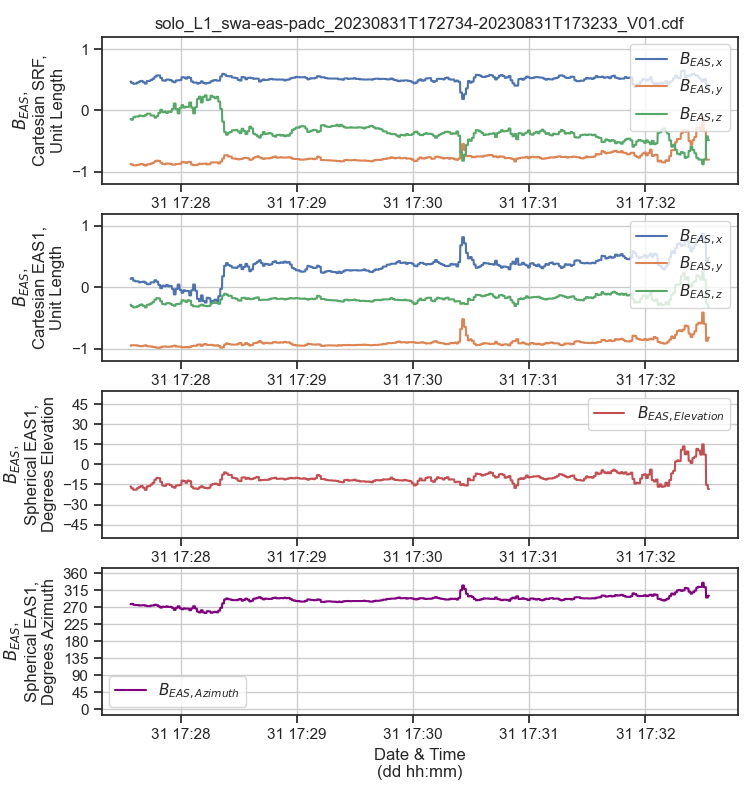
\includegraphics[width=1.05\linewidth]{figures/Transformation Example.png}
    \caption{Example \(B_{EAS}\) data from 31st August 2023. Top panel: Default cartesian \(B_{EAS}\) in SRF frame. 2nd panel: Cartesian \(B_{EAS}\) in EAS1 frame. 3rd panel: Elevation for spherical \(B_{EAS}\) in EAS1 frame. bottom panel: Azimuth for spherical \(B_{EAS}\) in EAS1 frame. The radius in spherical coordinates is not shown because all time series vectors are of length unity.}
    \caption*{Image Source: Author's own work}
    \label{fig: trans example}
\end{figure}

\(B_{EAS}\) and \(B_{MAG}\) are both acquired from SOAR in cartesian SRF coordinates. This is contrasted with data in cartesian radial-tangent-normal (RTN) coordinates (which are also provided for MAG\cite{soar}), where the \q{x-axis} is oriented radially away from the Sun, the \q{z-axis} is oriented towards the north celestial pole, and the \q{y-axis} is tangent to a prograde orbit in the plane of the ecliptic, completing the triad. SRF coordinates correspond to the \q{S/C Frame} shown in Figure \ref{fig: EAS schematic}, which is approximately equivalent to RTN coordinates with the \q{x and y} axes inverted. However, this equivalence depends on Solar Orbiter's pointing accuracy, meaning that transformations between rigidly-coupled onboard reference frames (e.g. SRF and the EAS Instrument frame in Figure \ref{fig: EAS schematic}) are generally expected to be more consistent than transformations between onboard reference frames and celestial reference frames such as RTN\cite{erofeev2019}.
\\

To determine the effect of \(B_{EAS}\) and \(B_{MAG}\) on EAS elevation/azimuth binning, these time series had to be converted from cartesian SRF coordinates to spherical EAS1/EAS2 coordinates in terms of radius and elevation and azimuth angles, where the head should be chosen such that \(B_{EAS}\) and/or \(B_{MAG}\) lie within that head's FOV. This was calculated in the following order: Cartesian SRF \(\rightarrow\) Cartesian EAS1/2 \(\rightarrow\) Spherical EAS1/2. This order was chosen because SOAR provides \q{EAS\textit{X}\_TO\_SRF} transformation matrices packaged with level 2 EAS data CDF files published under \q{solo\_L2\_swa-eas\textit{X}-nm3d-dnf\_\textit{YYYYMMdd}T\textit{hhmmss}-\textit{YYYYMMdd}T\textit{hhmmss}\_V01.cdf} where \textit{X} is the EAS head number (1 or 2). Despite being packaged with timestamped CDF files, these transformation matrices do not appear to change over time (nor should they be expected to change over time). The matrices can be trivially inverted to enable a Cartesian SRF \(\rightarrow\) Cartesian EAS1/2 transformation. The default and inverted forms are shown in Table \ref{tab: EASX to SRF}, as would be expected geometrically based on Figure \ref{fig: EAS schematic}.

\begin{table}[h!]
    \centering
    \(
    \begin{array}{cc}
        \text{EAS1 to SRF} & \text{SRF to EAS1} \\
        \begin{bmatrix}
        0 & -\frac{\sqrt{2}}{2} & +\frac{\sqrt{2}}{2}\\
        0 & +\frac{\sqrt{2}}{2} & +\frac{\sqrt{2}}{2}\\
        -1 & 0 & 0\\
        \end{bmatrix} &
        \begin{bmatrix}
        0 & 0 & -1\\
        -\frac{\sqrt{2}}{2} & +\frac{\sqrt{2}}{2} & 0\\
        +\frac{\sqrt{2}}{2} & +\frac{\sqrt{2}}{2} & 0\\
        \end{bmatrix}
        \\
        \\
        \text{EAS2 to SRF} & \text{SRF to EAS2} \\
        \begin{bmatrix}
        0 & -\frac{\sqrt{2}}{2} & +\frac{\sqrt{2}}{2}\\
        0 & -\frac{\sqrt{2}}{2} & -\frac{\sqrt{2}}{2}\\
        -1 & 0 & 0\\
        \end{bmatrix} &
        \begin{bmatrix}
        0 & 0 & -1\\
        -\frac{\sqrt{2}}{2} & -\frac{\sqrt{2}}{2} & 0\\
        +\frac{\sqrt{2}}{2} & -\frac{\sqrt{2}}{2} & 0\\
        \end{bmatrix}
        \\
        
    \end{array}
    \)\\
    \caption{A table of transformation matrices between SRF and EAS1/2 coordinates in cartesian space. The matrices in the left column were found on SOAR (in reality, \(\pm\sqrt{2}/2\) was approximated as \(\pm0.707\) on SOAR).} 
    \label{tab: EASX to SRF}
\end{table}

% in particular, the \textit{CartesianRepresentation(x,y,z)} object with the \textit{.represent()} method

Once in the EAS1/2 frame, the Cartesian EAS1/2 \(\rightarrow\) Spherical EAS1/2 transformation was calculated using the \textit{astropy} library for Python\cite{astropy2013}\cite{astropy2018}\cite{astropy2022}. Figure \ref{fig: trans example} shows an example of normalised \(B_{EAS}\) data from 31st August 2023 at each stage of transformation from unit cartesian SRF to unit spherical coordinates in the EAS1 frame. Since the \Beas\ vector time series is normalised from the start, a time series of the radius in spherical coordinates would be trivial and is not shown. In Figure \ref{fig: trans example}, the x-axis, y-axis, and z-axis in the top panel (cartesian SRF) appear to align most closely with the z-axis (+ an offset), the y-axis (+ an offset), and the opposite of the x-axis in the 2nd panel (cartesian EAS1) respectively. This is also expected based on the \q{S/C} and \q{EAS 1 Science} frames in Figure \ref{fig: EAS schematic}, further validating the matrices in Table \ref{tab: EASX to SRF}.
\\


\section{Preliminary \(B_{EAS}\)-\(B_{MAG}\) Comparison: Method}
As described in the author's earlier work, a preliminary comparison was performed between \(B_{EAS}\) and \(B_{MAG}\) from a small set of arbitrarily selected periods of Burst Mode data to justify the creation of a completeness score\cite{dickson2024}.
\\

\(B_{EAS}\) time series are stored in EAS burst mode CDF files under \q{EPOCH} for the time axis and \q{SWA\_EAS\_MagDataUsed} for the series axis. Similarly, \(B_{MAG}\) time series are stored in MAG SRF normal mode CDF files under \q{EPOCH} and \q{B\_SRF} respectively. Every \q{B\_SRF} vector was normalised before comparison with \(B_{EAS}\). The dot product between \(B_{EAS}\) and \(B_{MAG}\) vectors gives the angular offset between them. This angle was calculated for every vector in a few randomly chosen time series, yielding the results and discussion presented in Section \ref{prelim results}, confirming the risk of PAD incompleteness for a few example datasets to justify the eventual development of a completeness metric. 

\section{Simulating EAS Burst Mode Steering} \label{sim steering - method}

To better understand sources of error in Burst Mode data, the Burst Mode steering algorithm was simulated in Python using \(B_{EAS}\) vectors, Table \ref{fig: trans example}, and the latest published binning tables shown in Appendix \ref{appendixlabel1}. As per Section \ref{EAS Burst Mode}, the algorithm first requires a comparison between \(B_{EAS}\) and both EAS head aperture center planes in SRF coordinates, equivalent to their z-axes + 90\degree\ elevation in their respective EAS coordinates. This algorithm can be summarised as follows: 

\begin{enumerate}
    \item The angles between \(B_{EAS}\) and both EAS head aperture center planes are calculated.
    \item The smallest angle selects the EAS frame to which \(B_{EAS}\) is transformed, in spherical coordinates.
    \item The upper and lower bounds of the bin tables are compared to the elevation and azimuth angles of each vector in the spherical EAS frame until their correct bins are found.
\end{enumerate}

The anti-parallel vector to \(B_{EAS}\) is also determined and binned, resulting in two selected elevation bins. 
To validate the simulated binning algorithm, the time series for \(B_{EAS}\) can be plotted against the selected bin centers and upper and lower bounds. If head-selection has been performed correctly, then the \(B_{EAS}\) elevation component should never exceed \(\pm45\degree\). The results of this approach to validation were positive and are presented in Section \ref{sim steering}.
\\

The most direct way to validate the algorithm is to compare the simulated bins and heads selected to the actual bins and heads selected for a given dataset. EAS level 1 Burst Mode CDF data files on SOAR provide this information. The variable \q{SWA\_EAS\_EasUsed} contains a time series indicating the head selected (0 for EAS1, 1 for EAS2). \q{SWA\_EAS\_ElevationUsed} contains a 2D time series with the bin indices (0-15) of the elevation bins selected for parallel and anti-parallel \(B_{EAS}\). \q{SWA\_EAS\_ELEVATION}, \q{SWA\_EAS\_ELEVATION\_delta\_lower}, and \q{SWA\_EAS\_ELEVATION\_delta\_upper} contain 2D time series with the actual bin centers and boundaries used for the selected elevation bins (in degrees), for parallel and anti-parallel \(B_{EAS}\). In contrast, while there are similarly-named variables for azimuth (\q{SWA\_EAS\_AZIMUTH}, \q{SWA\_EAS\_AZIMUTH\_delta\_lower}, and \q{SWA\_EAS\_AZIMUTH\_delta\_upper}), these do not contain time series. Instead, the azimuth variables contain the constant bin center and delta data found in Table \ref{tab: Bin Table EAS Azimuth July 2021}. Therefore, simulated azimuth binning cannot be verified this way. This is of no consequence to Burst Mode simulation because steering is only determined by elevation binning.
\\

The results of this approach to validation led to the discovery of an error in the memory of the SWA Data Processing Unit (SWA-DPU). These results are also presented in Section \ref{sim steering}.

\section{Visualisation for Bins and Vectors} \label{visualisation}
To facilitate the determination of Burst Mode data accuracy, a visualisation tool was developed for this project based on a plot produced by Owen et al (2021)\cite{owen2021}. This was the tool that was used to create Figures \ref{fig: all bins}, \ref{fig: normal - full contours}, and \ref{fig: normal - full contours + selection} in Section \ref{EAS PAD}. This visualisation is attractive because it concisely displays magnetic field vectors in SRF, circumventing the need to change coordinates following a sensor head change. The choice of SRF over RTN has been justified in Section \ref{coordinate systems}. This approach to visualisation also allows the difference in angular bin widths to be seen projected on to the sky, visualising each head and pixel's field of view along with \Beas\ vectors in a form that may facilitate a more intuitive determination of the ensuing effects on Burst Mode steering compared to other approaches.
\\

The visualisation was implemented in Python. The first step was to plot the grid of angular EAS bins in SRF space. Plotting the grid is easily (though inefficiently) accomplished in the EAS1/2 frame using spherical coordinates by simply plotting many closely-spaced points in straight lines along the upper and lower bounds of the elevation and azimuth bin tables (see Appendix \ref{appendixlabel1}). This step is described in detail with added excerpts of code from its implementation in Appendix \ref{appendixlabel2}. Plotting the parallel and anti-parallel magnetic field vectors seen in Figures \ref{fig: normal - full contours} and \ref{fig: normal - full contours + selection} was also relatively straightforward. Since both \(B_{EAS}\) and \(B_{MAG}\) are acquired from SOAR in SRF coordinates, they only had to be transformed to spherical coordinates and plotted with distinct markers to differentiate them. The markers used throughout this report are a diamond for the parallel vector and a square for the anti-parallel vector. \(B_{EAS}\) and \(B_{MAG}\) vectors are also differentiated by colour (green and purple respectively).
\\

To plot the contours of constant pitch angle at arbitrary pitch angles around these vectors involved adapting an algorithm written by Dr. Chris Owen in Interactive Data Language (IDL). The algorithm starts by constructing the transformation matrix \textit{M} from a cartesian reference frame whose z-axis is aligned with the magnetic field vector to cartesian SRF coordinates. \textit{M} is constructed using the elevation and azimuth for a magnetic field vector \(B\) in spherical SRF coordinates as per Equation \ref{eq: Matrix M}, where \(\theta=\textrm{(spherical SRF magnetic field elevation)}*\pi/180\degree\) and \(\phi=\textrm{(spherical SRF magnetic field azimuth)}*\pi/180\degree\).

\begin{equation} \label{eq: Matrix M}
    M=
    \begin{bmatrix}
    \cos{\phi}\cos{\theta} & -\sin{\phi} & -\cos{\phi}\sin{\theta}\\
    \sin{\phi}\cos{\theta} & \cos{\phi} & -\sin{\phi}\sin{\theta}\\
    \sin{\theta} & 0 & \cos{\theta}\\
    \end{bmatrix}
\end{equation}

From there, the proceeding algorithm can be summarised as follows:
\begin{enumerate}
    \item For a given contour with pitch angle \(\alpha\), calculate the angular length (conceptually similar to \q{circumference}) of the contour in spherical SRF coordinates. Multiply this by the angular point density to yield a number of phase angles \(\varphi\) around \(B\) with which to plot points along the contour. \(\varphi\) is analogous to azimuth in the \(B\)-aligned frame.
    \item Working in the \(B\)-aligned frame, for every phase angle \(\varphi\), construct the cartesian vector \(\vec{p}_B\) according to:
    \begin{equation} \label{eq: contour vector construction}
        \centerfloat
        \vec{p}_B=
        \begin{bmatrix}
        x_{\alpha,\varphi}\\
        y_{\alpha,\varphi}\\
        z_{\alpha,\varphi}\\
        \end{bmatrix}
        =
        \begin{bmatrix}
        \cos{\alpha}\\
        \sin{\alpha}\cos{\varphi}\\
        \sin{\alpha}\sin{\varphi}\\
        \end{bmatrix}
    \end{equation}
    \item Transform \(\vec{p}_B\) into \(\vec{p}_{SRF}\) in the cartesian SRF frame using \textit{M} according to:
    \begin{equation} \label{eq: contour vector transform}
        \vec{p}_{SRF}=M\vec{p}_B
    \end{equation}
    \item Transform \(\vec{p}_{SRF}\) to spherical SRF coordinates, and its elevation and azimuth angles can be plotted directly.
\end{enumerate}
\\

Following this algorithm to plot all vectors for all phase angles in the range \([0\degree,360\degree]\) with appropriate increments and all pitch angles in the range \([0\degree,180\degree]\) in 15\degree\ increments yields Figure \ref{fig: normal - full contours} when plotted alongside EAS bins and the \Beas\ vector itself for the appropriate date and time.
\\

\begin{figure}[h!]
    \centering
    \centerfloat
    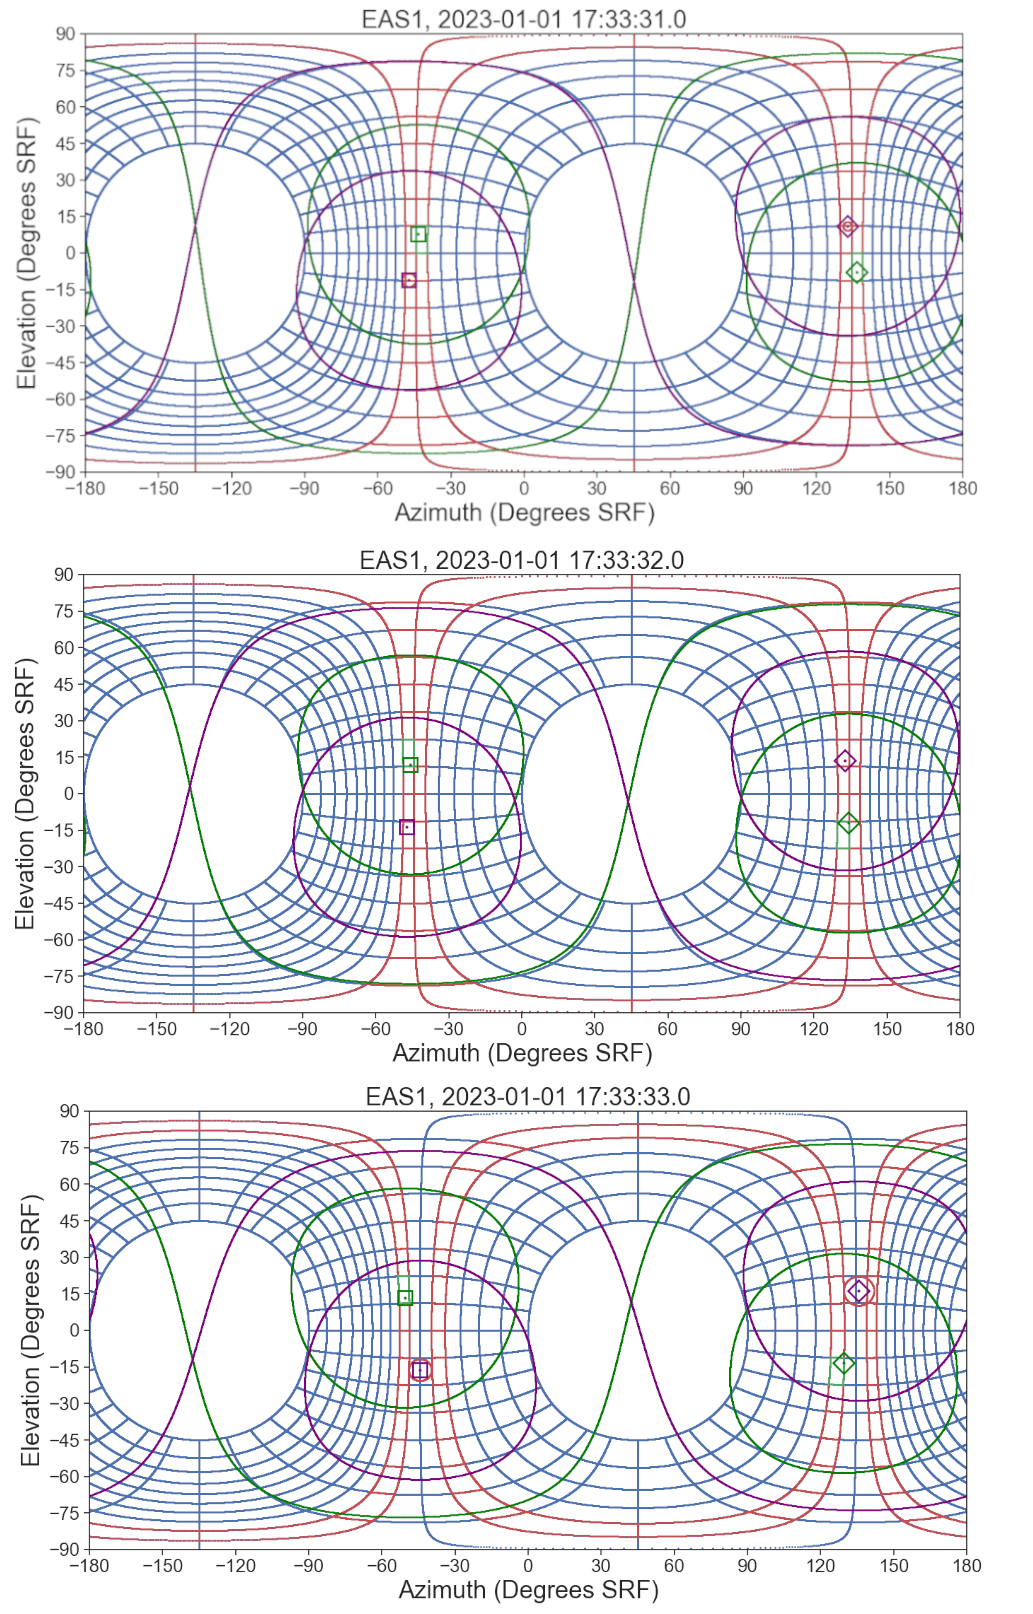
\includegraphics[width=0.84\linewidth]{figures/anim_example.png}
    \caption{Three frames of an animation produced by plotting \Beas\ and \Bmag\ data from 1st January 2023 along with pitch angle contours including loss contours, which are described in Section \ref{completeness}. Green represents \Beas\ and purple represents \Bmag. Diamond and square markers represent parallel and anti-parallel magnetic field vectors respectively. Top panel: Data from 17:33:31 UTC. Middle panel: Data from 17:33:32 UTC. Bottom panel: Data from 17:33:33 UTC.}
    \caption*{Image Source: Author's own work}
    \label{fig: animation example}
\end{figure}
\\
\newpage

As SOAR's magnetic field vector data comes in time series, this tool can also be used to visualise magnetic field variation over time in the form of an animation. Individual frames of an animation can be generated for every data point in a magnetic field time series, and then combined into a high-definition \textit{.gif} using the \textit{imageio} library for Python\cite{klein2024_imageio}\footnote{Other methods for composing \textit{.gif} files are available and may be more straightforward. One of the most straightforward methods is to use free online \q{image-to-gif} converters, but the resolution of \textit{.gif} files acquired by this method was found to be too low for this project's purposes.}. To play the animation at a realistic frame rate, the duration of each frame must be specified. For Burst Mode data, the duration is set to 0.125s, matching the time delay between successive time series vectors. Using data from 1st January 2023, three (non-consecutive) frames of such an animation, 1s apart, are included in Figure \ref{fig: animation example} for example.
\\

\section{S20 Link Latency} \label{S20 method}
It is possible that some of the \(B_{EAS}\)-\(B_{MAG}\) discrepancy can be attributed to latency over the S20 inter-instrument data link\cite{owen2021}.  This latency may be particularly noticeable on 1/8th second timeframe during periods of heavy data traffic\cite{owen2021}. If noticeable, then the latency is expected to cause a time delay between \(B_{EAS}\) and \(B_{MAG}\) where \(B_{MAG}\) leads by at least \(\sim\)0.125s. One approach to measuring this time delay is to perform a cross-correlation analysis between \(B_{EAS}\) and \(B_{MAG}\)\cite{hanus2019}); in principle, a cross-correlation function (CCF) takes a domain of time delays as input and the delay that gives the strongest correlation between the two time series can be selected to represent the latency. The principle behind this approach is well-illustrated by Figure \ref{fig: Hanus CCF} by Hanus et al\cite{hanus2019} for two 1D time series \(x(t)\) and \(z(t)\) and latency \(\tau_0\).
\\

\begin{figure}[h!]
    \centering
    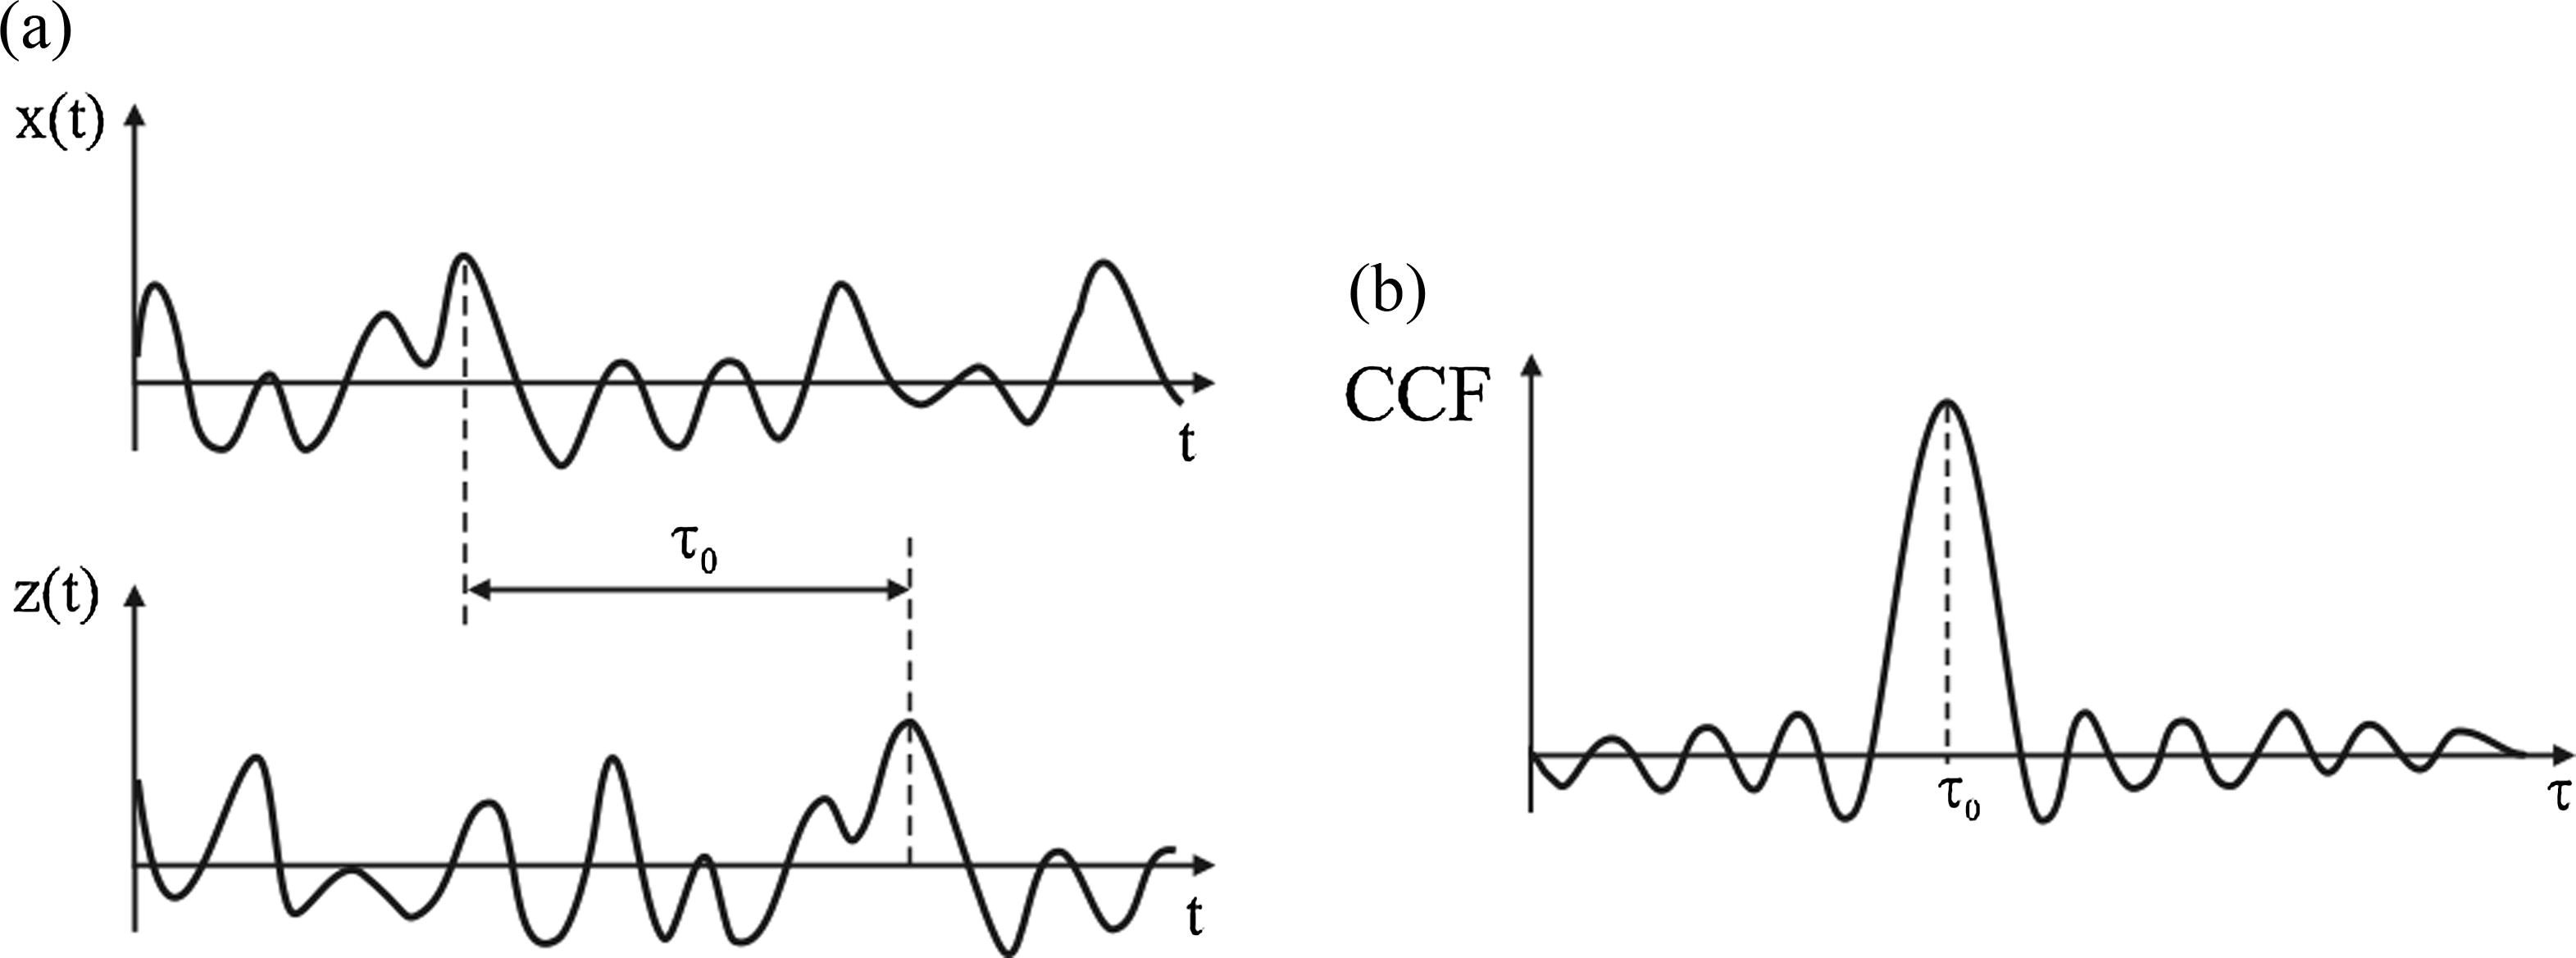
\includegraphics[width=1\linewidth]{figures/hanus diagram.jpg}
    \caption{Two figures illustrating CCF time delay determination. (a): Two arbitrary time series \(x(t)\) and \(z(t)\), which are well-approximated as identical time series with a time delay \(\tau_0\) between them. (b): A plot of the CCF applied to \(x(t)\) and \(z(t)\), showing maximum correlation at the time delay \(\tau_0\), representing the latency.}
    \caption*{Image Source: Hanus et al\cite{hanus2019}}
    \label{fig: Hanus CCF}
\end{figure}

A version of the cross-correlation approach was implemented in Python to calculate the S20 latency \(\tau_{S20}\). The \textit{scipy} library for Python provides a wide range of signal processing methods and functions, including CCFs\cite{2020SciPy}. Given two 1D arrays of data, the discrete CCF between them can be determined using the \textit{scipy.signal.correlate()} method\cite{2020SciPy}. The discrete CCF generated by this method is an approximation of a theoretical CCF between two complex, 1D functions \(f(t)\) and \(g(t)\) over time \textit{t}. The CCF, sometimes denoted \q{\(f\star g\)}, is generated by convolving \(g(t)\) with the complex conjugate of \(f(t)\), \(\overline{f}(t)\) according to:

\begin{equation} \label{eq: continuous CCF}
    f\star g=\overline{f}(-t)\ast g(t)
\end{equation}

where convolution is denoted by \q{\(\ast\)}\cite{bracewell1986}\cite{CCFs}. Convolution is defined by:

\begin{equation} \label{eq: convolution}
    (f\ast g)(t)=\int_{-\infty}^{\infty}f(\tau)g(t-\tau)d\tau
\end{equation}

where \(\tau\) denotes the continuously-variable displacement in time between \(f(t)\) and \(g(t)\)\cite{CCFs}, also known as the \textit{lag}. Combining Equations \ref{eq: continuous CCF} and \ref{eq: convolution} and changing integration variables from \textit{t} to \(\tau\) yields Equation \ref{eq: continuous CCF integral} for the cross-correlation in terms of \(\tau\):

\begin{equation} \label{eq: continuous CCF integral}
    (f\star g)(\tau)=\int_{-\infty}^{\infty}\overline{f}(t)g(t+\tau)dt
\end{equation}

Equation \ref{eq: continuous CCF integral} can be expressed in its discrete form in terms of discrete functions \(f(t)\) and \(g(t)\), yielding:

\begin{equation} \label{eq: discrete CCF}
    \textrm{CCF}\equiv(f\star g)(\tau)=\sum_{-\infty}^{\infty}\overline{f}(t)g(t+\tau)
\end{equation}

This is the definition of \q{CCF} that will be used for the remainder of this section\cite{2020SciPy}\cite{rabiner1978}. The translation of Equation \ref{eq: discrete CCF} into Python is given by \textit{scipy.signal.correlate()}. The array of lags \(\tau\) is generated by \textit{scipy.signal.correlation\_lags()}, which depends on the sample rate of \(f(t)\) and \(g(t)\) to define the timescale of \(\tau\). For this project, that is equivalent to the EAS Burst Mode sample rate of 8Hz. With the CCF and the array of lags, the latency \(\tau_0\) can be estimated by calculating the maximum of the CCF and finding its corresponding lag.
\\

\begin{figure}[h!]
    \centering
    \centerfloat
    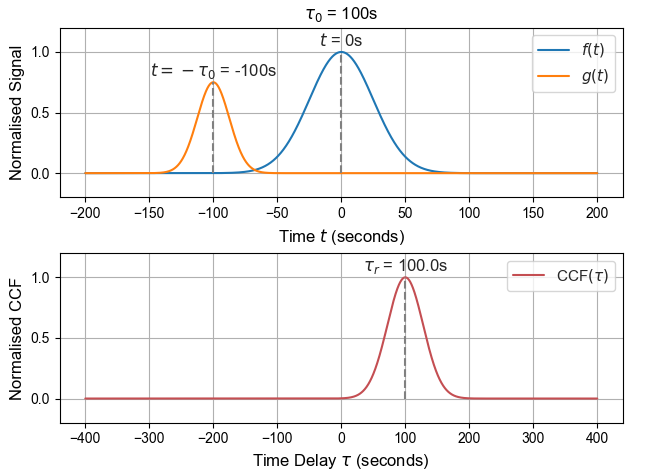
\includegraphics[width=1\linewidth]{figures/Time Delay Tests - Clean.png}
    \caption{Two figures illustrating the time delay algorithm for dummy data. Top panel: Normalised dummy time signals \(f(t)\) and \(g(t)\) plotted over 400s with a time delay \(\tau_0\) between them. The peaks of \(f(t)\) and \(g(t)\) are labelled with their time values. Bottom panel: The CCF of \(f(t)\) and \(g(t)\) plotted over 800s of time delays \(\tau\). The peak of the CCF is labelled with its value for the time delay \(\tau_r\approx \tau_0\).}
    \caption*{Image Source: Author's own work}
    \label{fig: time delay tests - clean}
\end{figure}

This time delay algorithm was implemented and validated using dummy time series data consisting of two Gaussian signals, \(f(t)\) and \(g(t)\) as shown in the upper half of Figure \ref{fig: time delay tests - clean}. \(f(t)\) has amplitude \(a_f=1\) and standard deviation \(\sigma_f=25\)s, and \(g(t)\) has \(a_g=0.75\) and \(\sigma_g=12.5\)s. \(f(t)\) and \(g(t)\) are distributed over 400s with \(N=3200\) data points to simulate the Burst Mode sample rate of 8Hz. There is a delay \(\tau_0=100\)s between \(f(t)\) and \(g(t)\), with \(f(t)\) in the lead. In the lower half of Figure \ref{fig: time delay tests - clean}, the calculated and normalised CCF is plotted against the array of lags over twice the duration of \(f(t)\) and \(g(t)\), showing a clear Gaussian peak at the value of \(\tau_0\) that it recovered from the comparison of \(f(t)\) and \(g(t)\), which is denoted \(\tau_r\). Figure \ref{fig: time delay tests - clean} shows reassuring results, correctly recovering a value of \(\tau_r=100.000\textrm{s}=\tau_0\). 
\\

The issue now is to determine the uncertainty in the calculated value. There is not much consensus on the \q{correct} approach to measuring the uncertainty CCF lags\cite{peterson1998}\cite{efron1992}. Peterson et al (1998) suggest Monte Carlo simulations of many small variations on the same cross-correlation to evaluate the sensitivity of the lag solution to individual data points. Specifically, they suggest a statistical test where the time series subject to the CCF is reduced to a large number of randomly selected subsets of the original dataset, each of which is shrunken by a factor \(\sim 1/e \approx0.37\). These subsets are each subjected to the CCF in the same way as before, allowing the calculation of a mean and standard deviation which provide a conservative estimate of the uncertainty. The principle behind this method inspired the implementation of a Python algorithm for calculating the uncertainty on the lag. The algorithm can be summarised as follows for arrays to be correlated, \(f\) and \(g\):
\begin{enumerate}
    \item Define two empty arrays \(f_i\) and \(g_i\). These will be the subset arrays.
    \item Starting from 0, take a random integer \q{step} through the indices of the arrays \(f\) and \(g\) and select their corresponding values to append to \(f_i\) and \(g_i\) respectively. The average length of the step should be \(\approx e\) to get the \(\sim1/e\) shrink factor (e.g. the first values might be randomly distributed around \(f(3)\) and \(g(3)\)).
    \item Repeat step 2 until the end of \(f\) and \(g\) is reached, and then cross-correlate \(f_i\) and \(g_i\) to calculate \(\tau_r\), dividing the sample rate by the average step length to reflect the subset's new data rate.
    \item Repeat steps 1 through 3 over \textit{M} iterations, and calculate the mean time delay \(\tau_r\) and standard deviation \(\sigma\) of the resulting collection of \(\tau_r\) values. \(\sigma\) is said to represent the uncertainty in \(\tau_r\).
\end{enumerate}
\\

\begin{figure}[h!]
    \centering
    \centerfloat
    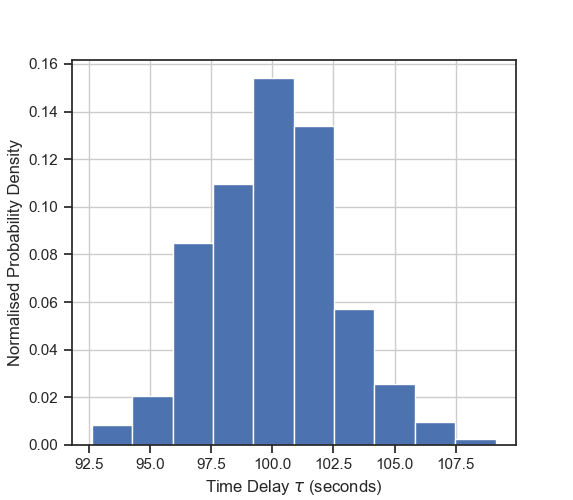
\includegraphics[width=0.8\linewidth]{figures/dummy hist.png}
    \caption{A histogram of the probability density function describing the \(M=1000\) simulations used to calculate the uncertainty in \(\tau_r\) for the dummy data used in Figure \ref{fig: time delay tests - clean}. There are 10 equally-spaced time delay bins.}
    \caption*{Image Source: Author's own work}
    \label{fig: dummy hist}
\end{figure}

\noindent The algorithm was validated using the same dummy data shown in Figure \ref{fig: time delay tests - clean}. In this case, the average step length was set to 3, and the random steps were calculated using a uniform random variable in the inclusive range \((1,5)\). After \(M=1000\) iterations, a value of \(\tau_r=100.0\textrm{s}\pm2.6\textrm{s}\) was acquired. A probability density histogram resulting from the Monte Carlo simulation is shown in Figure \ref{fig: dummy hist}. While an uncertainty of \(\pm2.6\textrm{s}\) is too small to be displayed on a plot of the same scale as Figure \ref{fig: time delay tests - clean}, it is significantly larger than the time resolution of 8Hz magnetic field data. Given that the dummy data used in this exercise are, by design, much \q{cleaner} than real magnetic field time series, this suggests a restrictive lower bound on the resolution of S20 data link latency determination using this method. The results of further experiments using real magnetic field data are presented in Section \ref{S20 Link Latency}.

% Further validation tests were performed by adding Gaussian noise to \(f(t)\) and \(g(t)\) with an arbitrary scale \(\sigma_n=0.05\). This was meant to evaluate the algorithm's performance in response to more realistic, non-uniform signals. An example of these tests is shown in Figure \ref{fig: time delay tests - noisy}. 10,000 of these tests were performed, yielding a mean \(\langle\tau_r\rangle=99.965\)s with standard deviation \(\sigma=0.547\)s.

% \begin{figure}[h!]
%     \centering
%     \centerfloat
%     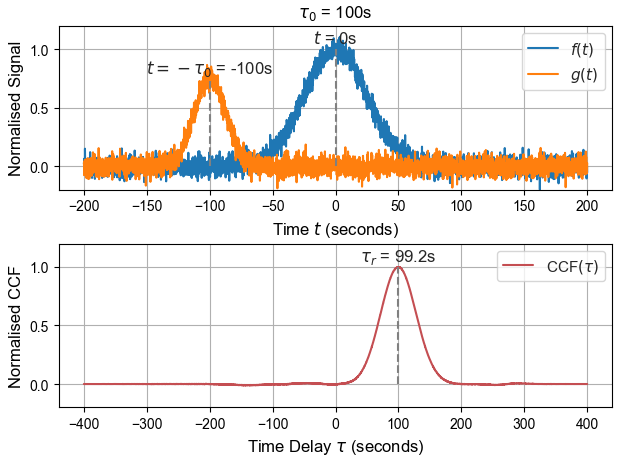
\includegraphics[width=1\linewidth]{figures/Time Delay Tests - Noisy.png}
%     \caption{Two more figures illustrating the time delay algorithm for the dummy data shown in Figure \ref{fig: time delay tests - clean} with added Gaussian noise. Top panel: \(f(t)\) and \(g(t)\) + Gaussian noise of scale \(\sigma_n=0.05\). Peaks labelled with time values. Bottom panel: The CCF of \(f(t)\) and \(g(t)\) + noise, peak labelled with \(\tau_r\).}
%     \caption*{Image Source: Author's own work}
%     \label{fig: time delay tests - noisy}
% \end{figure}

% Having been validated on dummy data, the next step is to apply this lag algorithm to real magnetic field time series.
